\subsection{Performance}

\begin{figure*}[t]

  \begin{subfigure}[b]{\textwidth}
          \centering
          
\includegraphics[width=0.4\textwidth]{data/legend.pdf}
  \end{subfigure}

  \begin{subfigure}[b]{0.5\textwidth}
      \centering
      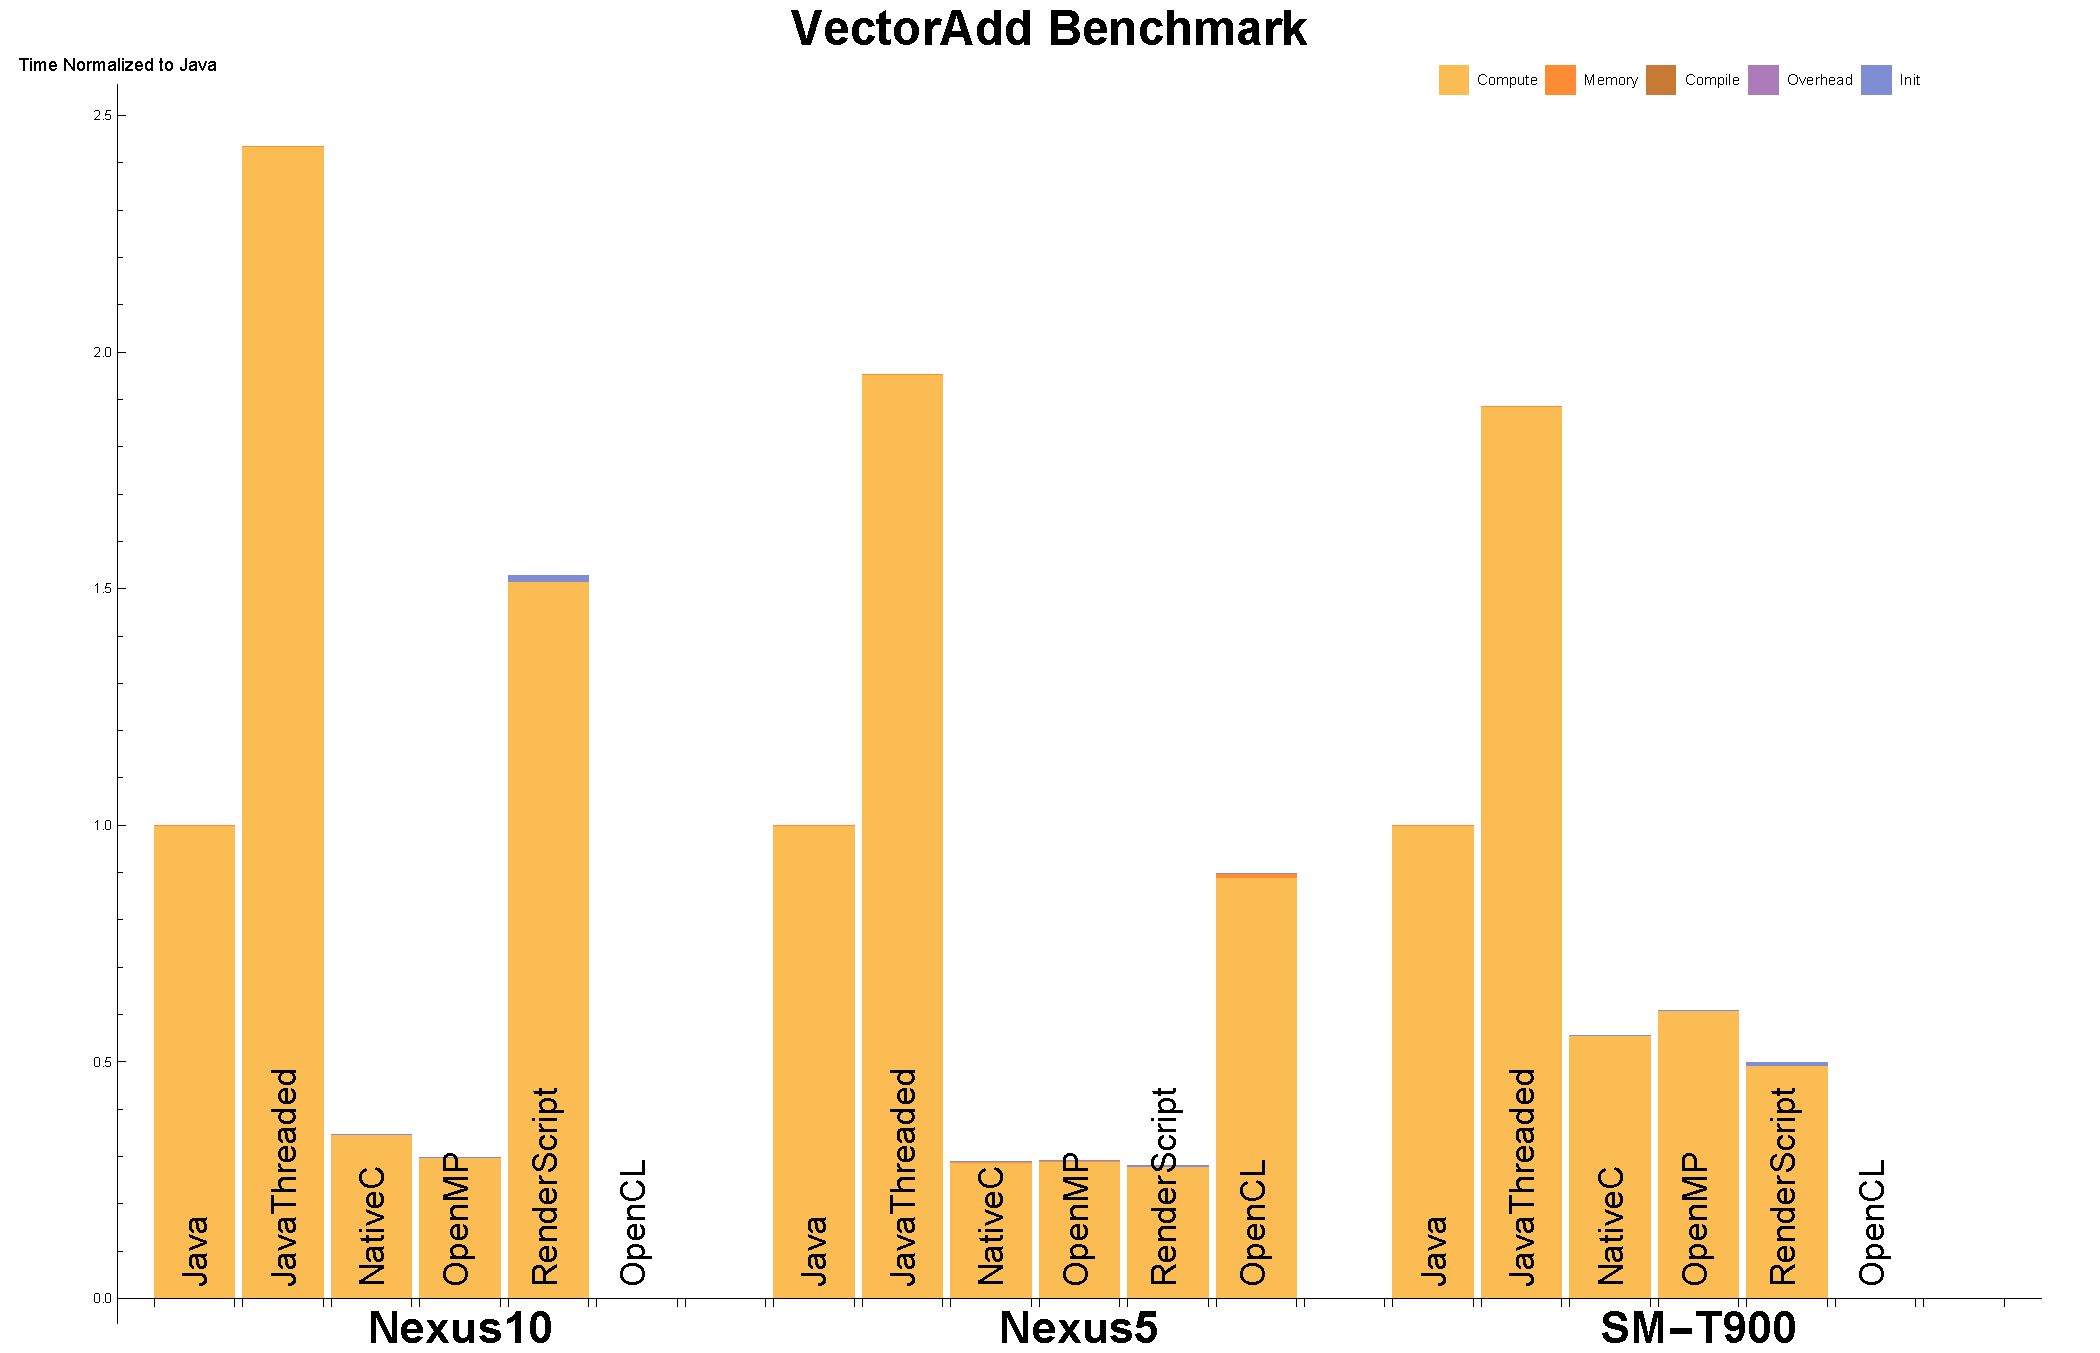
\includegraphics[width=0.9\textwidth]{data/VectorAdd_onecompute_time.pdf}
      \caption{VectorAdd}\label{fig:vectoradd}
  \end{subfigure}
  \begin{subfigure}[b]{0.5\textwidth}
      \centering
      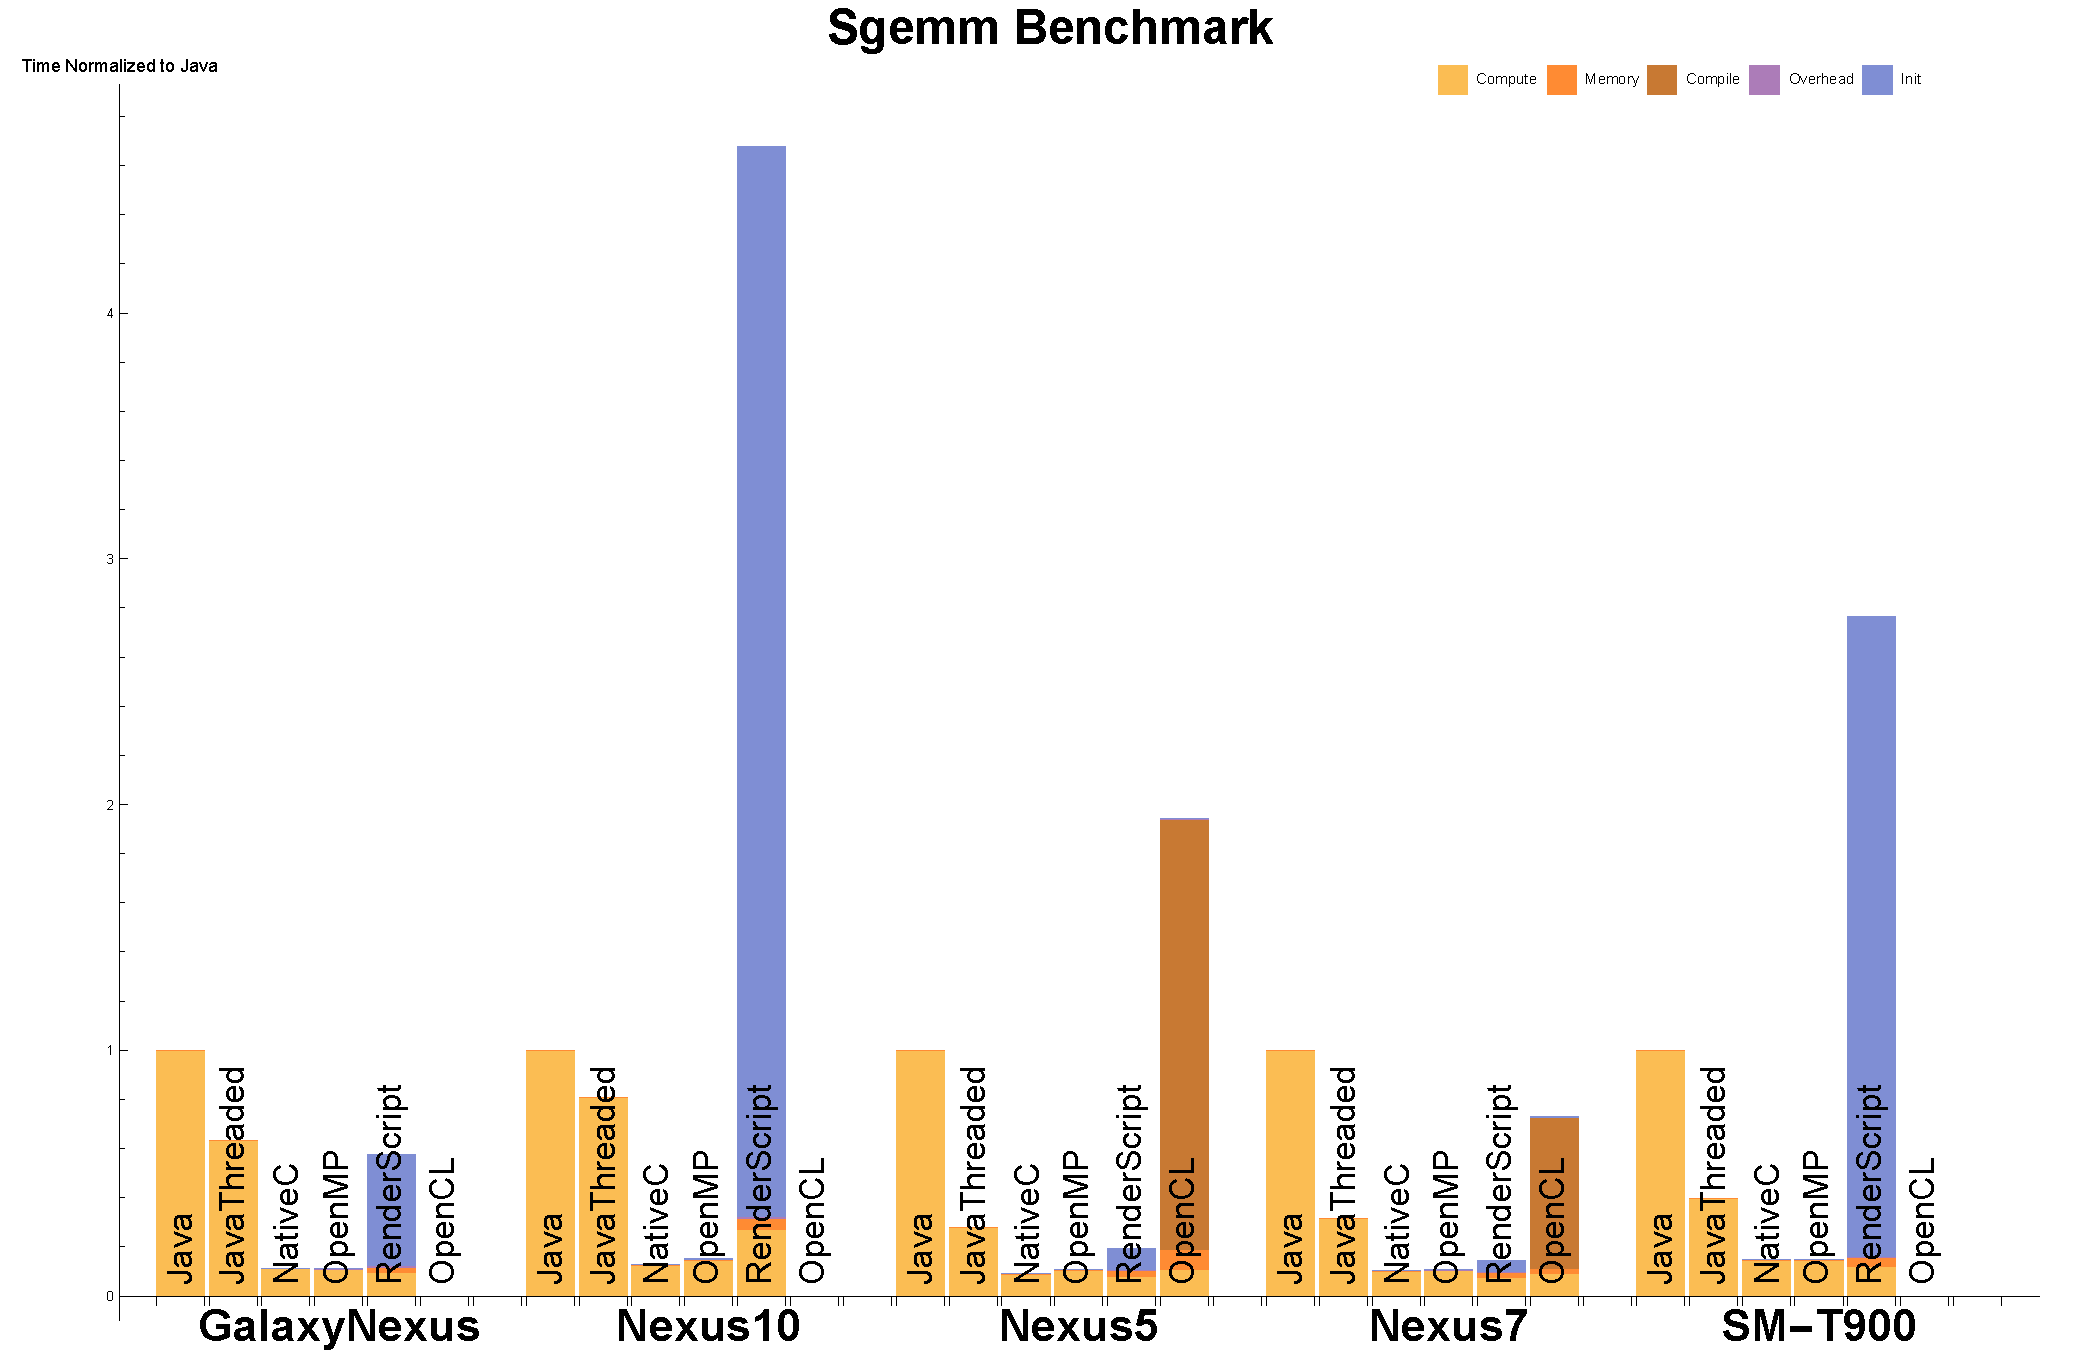
\includegraphics[width=0.9\textwidth]{data/Sgemm_onecompute_time.pdf}
      \caption{Sgemm}\label{fig:Sgemm}
  \end{subfigure}

  \begin{subfigure}[b]{0.5\textwidth}
      \centering
      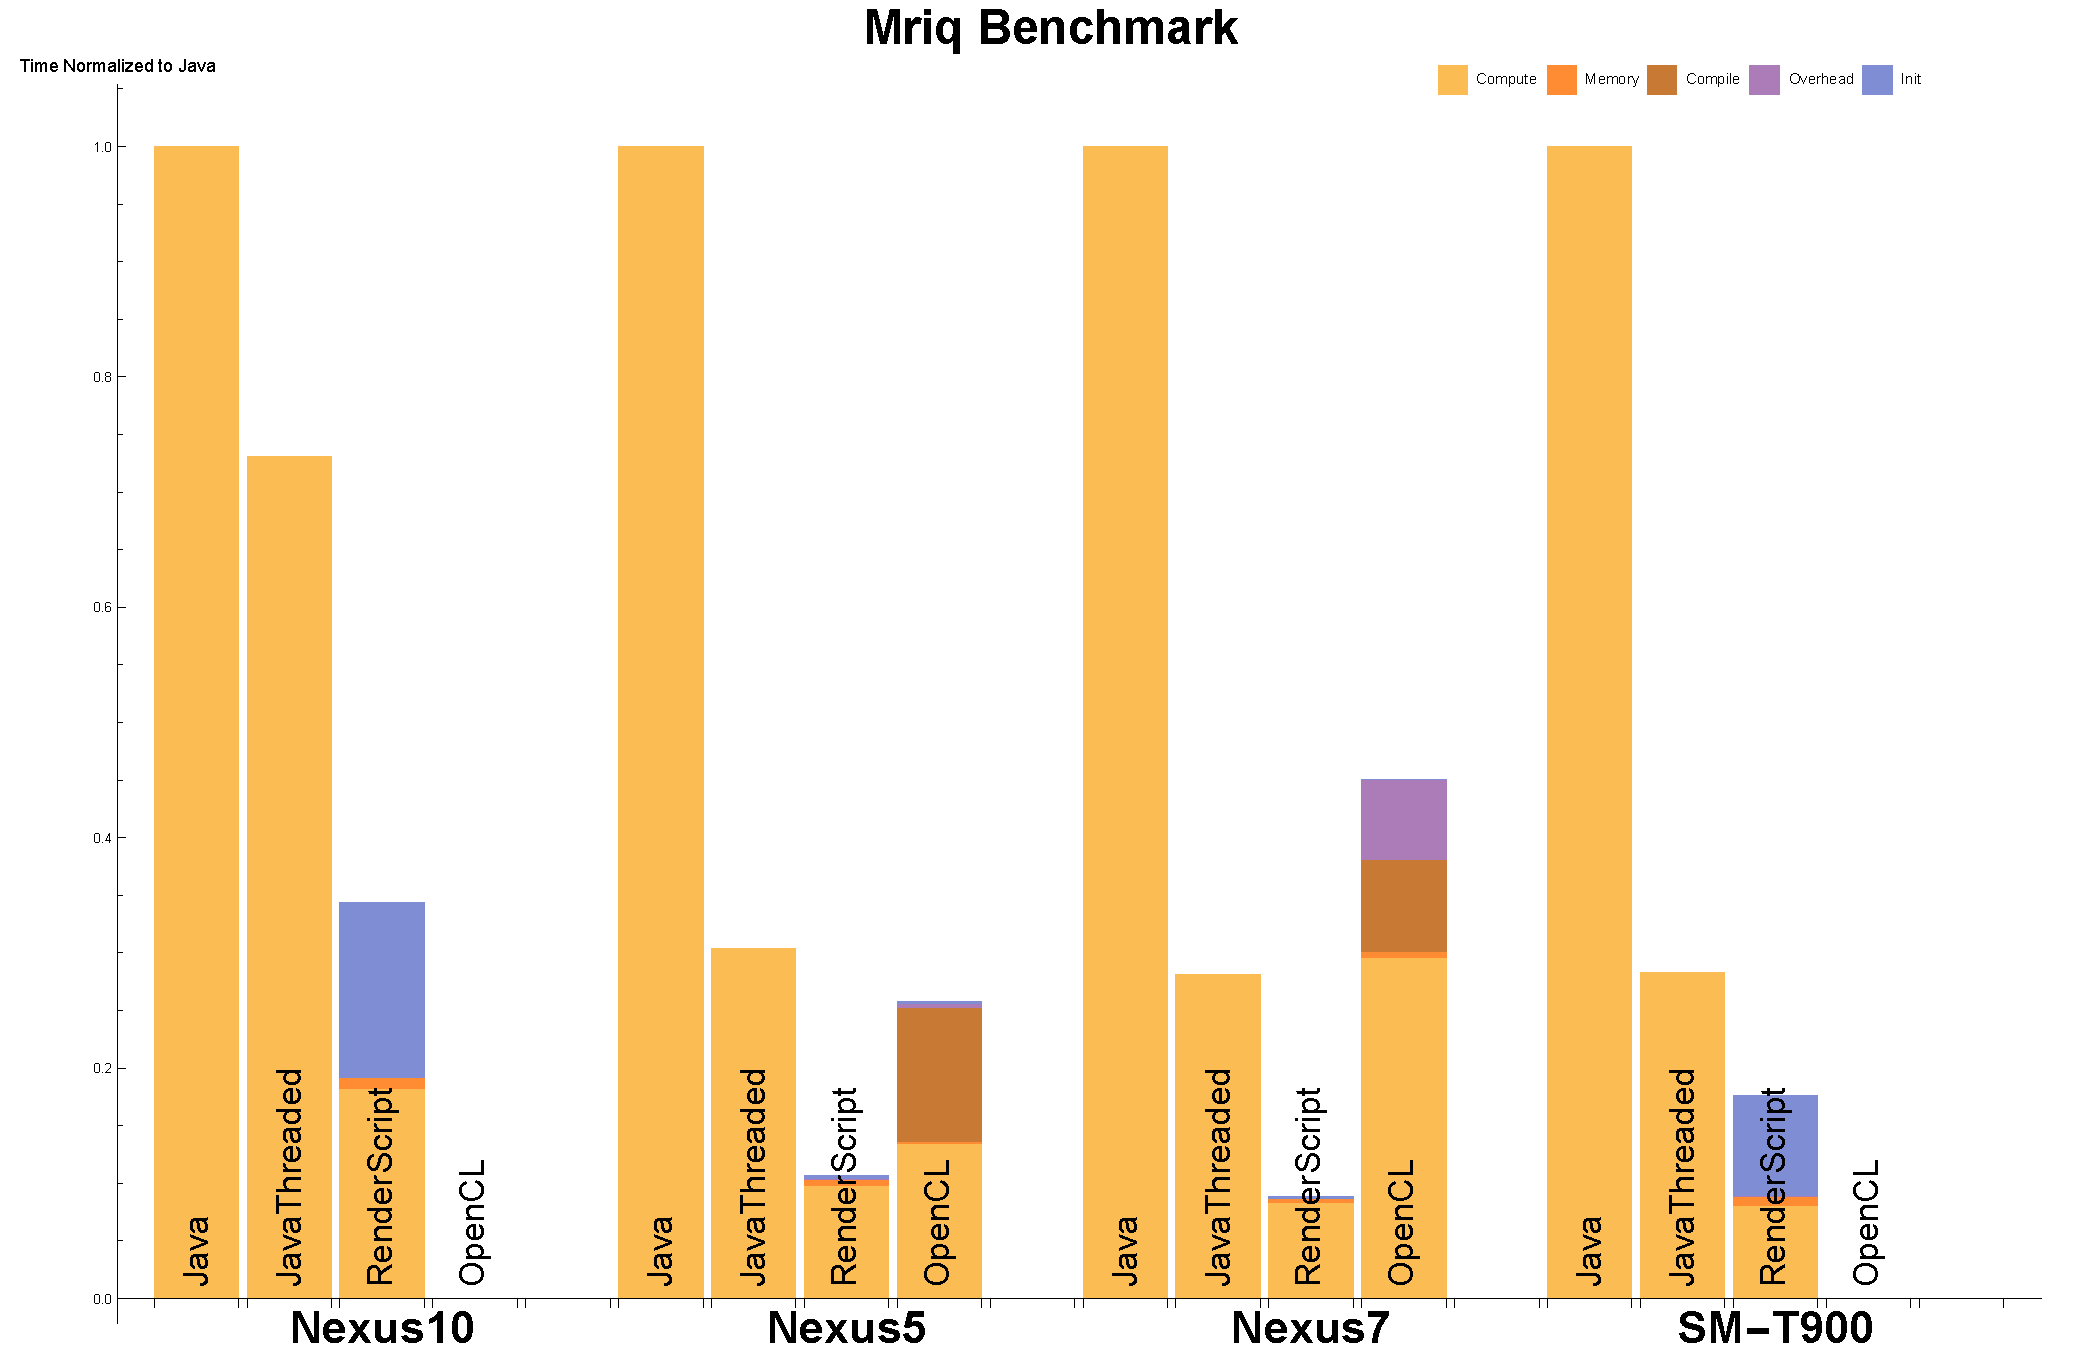
\includegraphics[width=0.9\textwidth]{data/Mriq_onecompute_time.pdf}
      \caption{MRIQ}
      \label{fig:MRIQ}
  \end{subfigure}
  \begin{subfigure}[b]{0.5\textwidth}
      \centering
      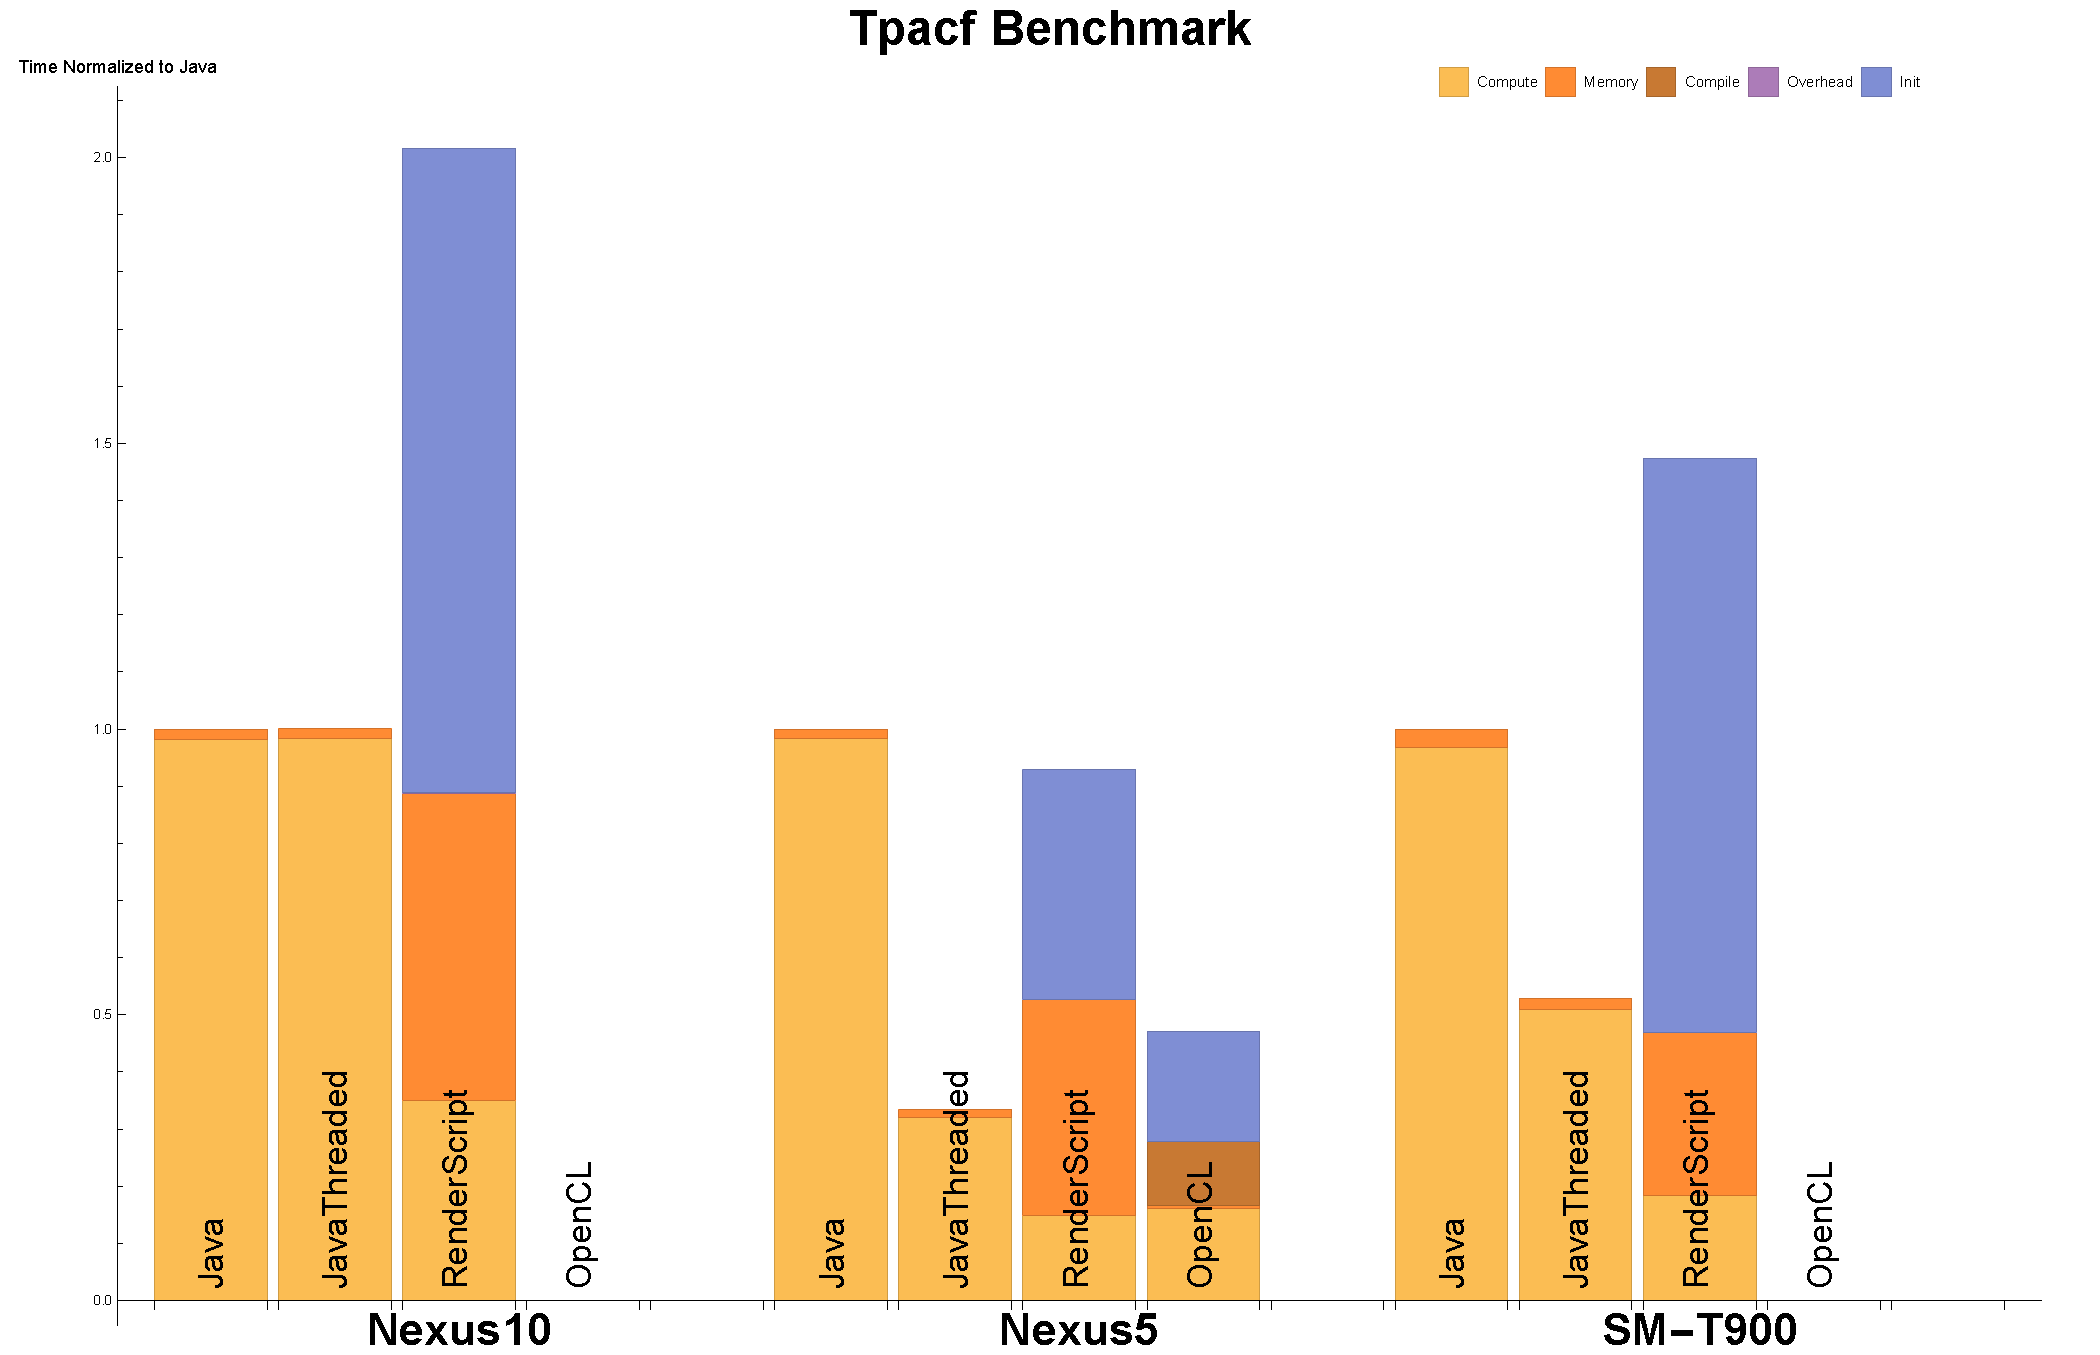
\includegraphics[width=0.9\textwidth]{data/Tpacf_onecompute_time.pdf}
      \caption{TPACF}
      \label{fig:TPACF}
  \end{subfigure}

  \begin{subfigure}[b]{0.5\textwidth}
      \centering
      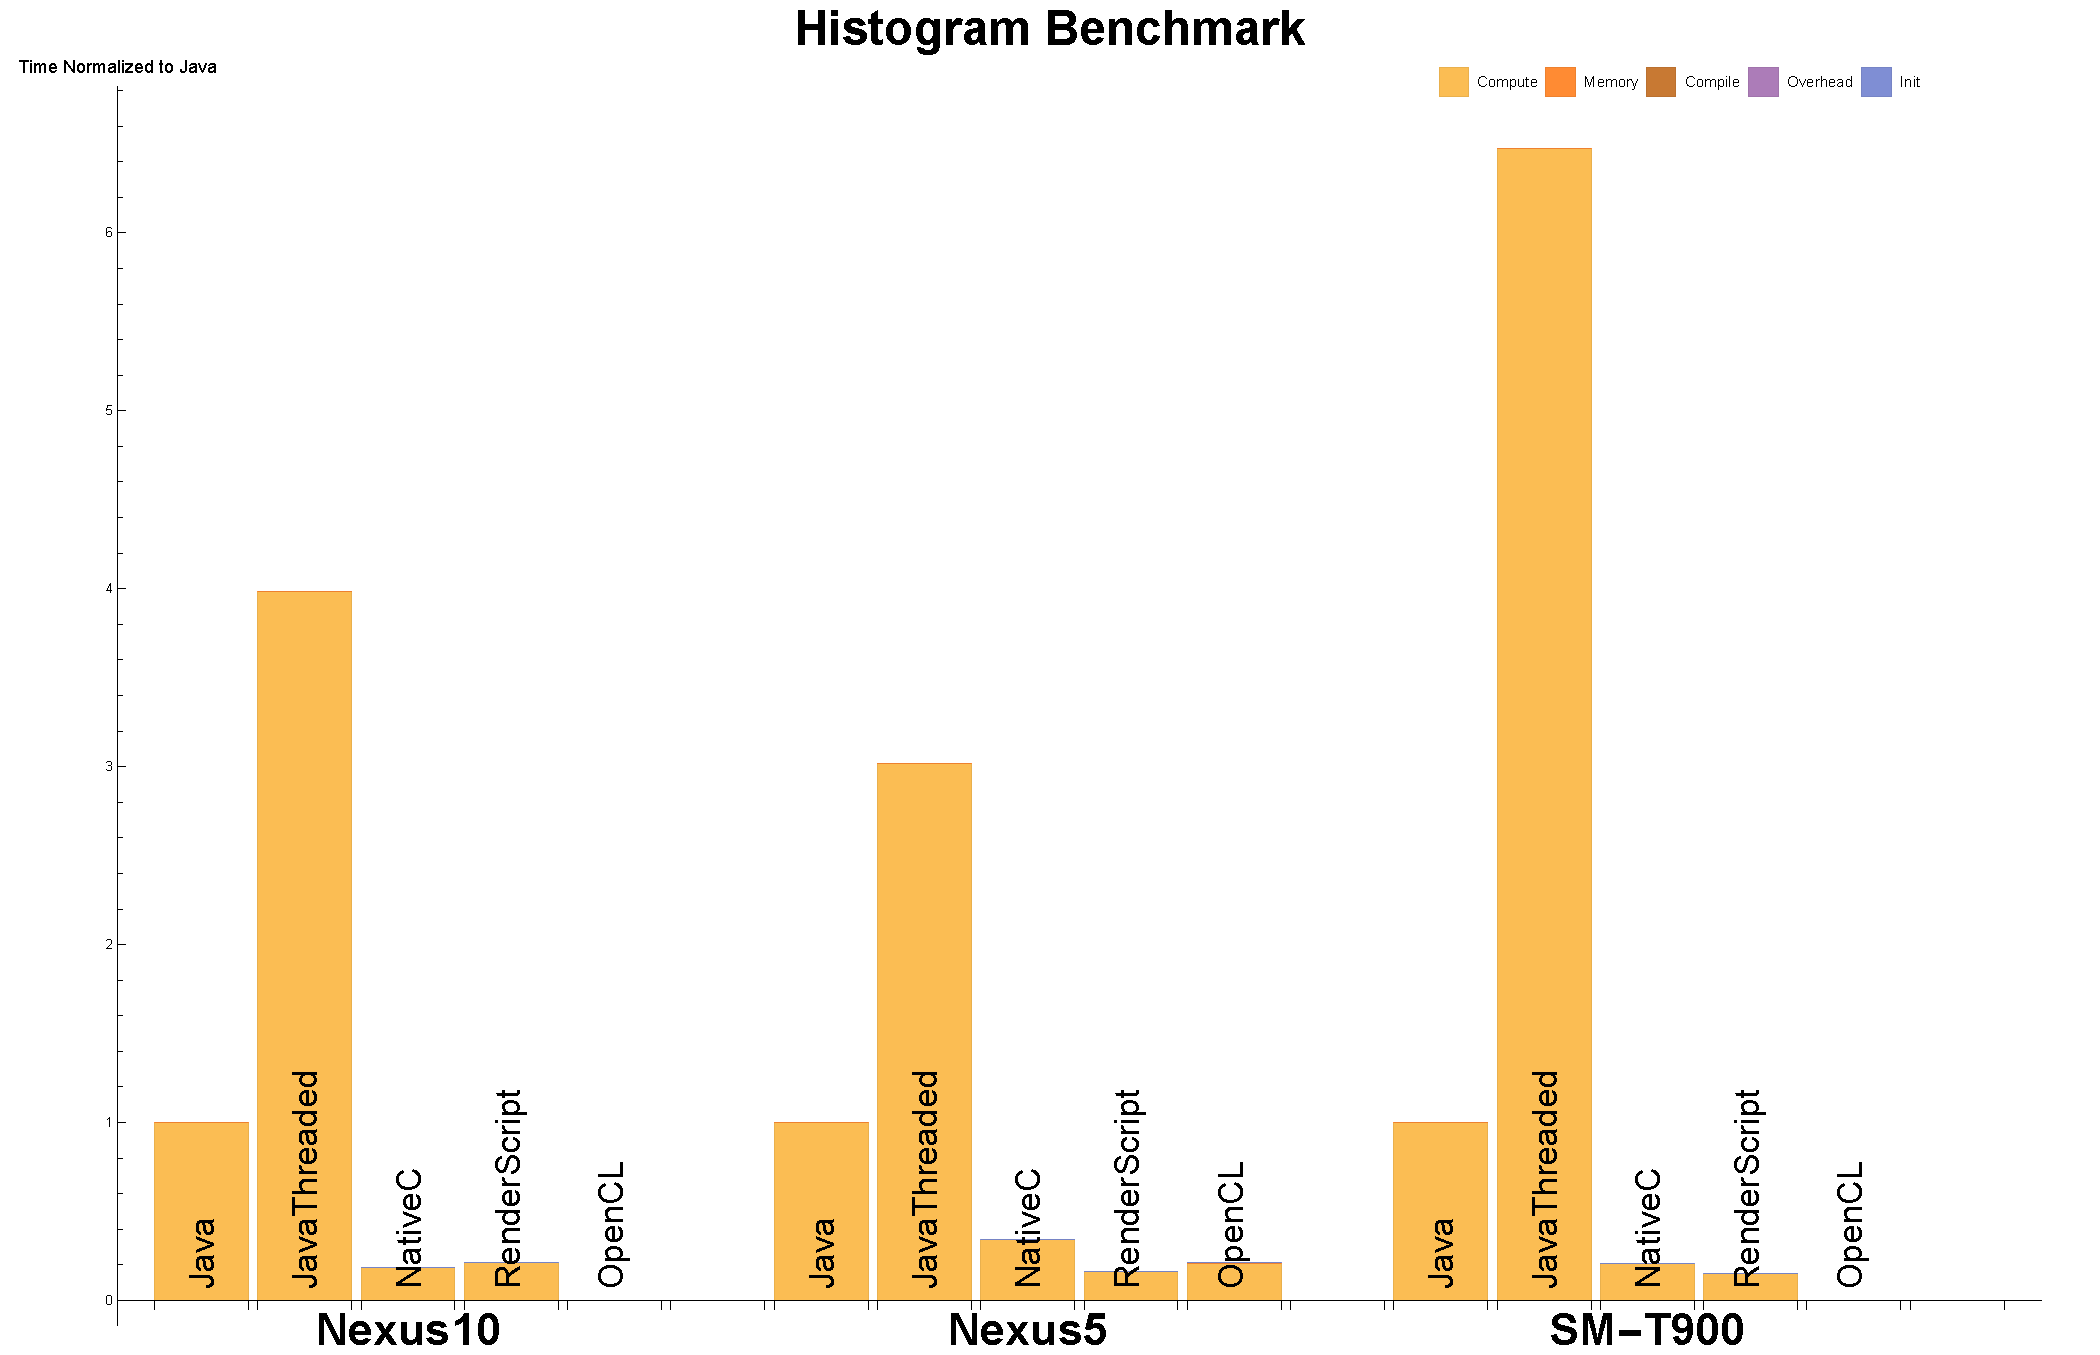
\includegraphics[width=0.9\textwidth]{data/Histogram_onecompute_time.pdf}
      \caption{Histogram}\label{fig:histo}
  \end{subfigure}
  \begin{subfigure}[b]{0.5\textwidth}
      \centering
      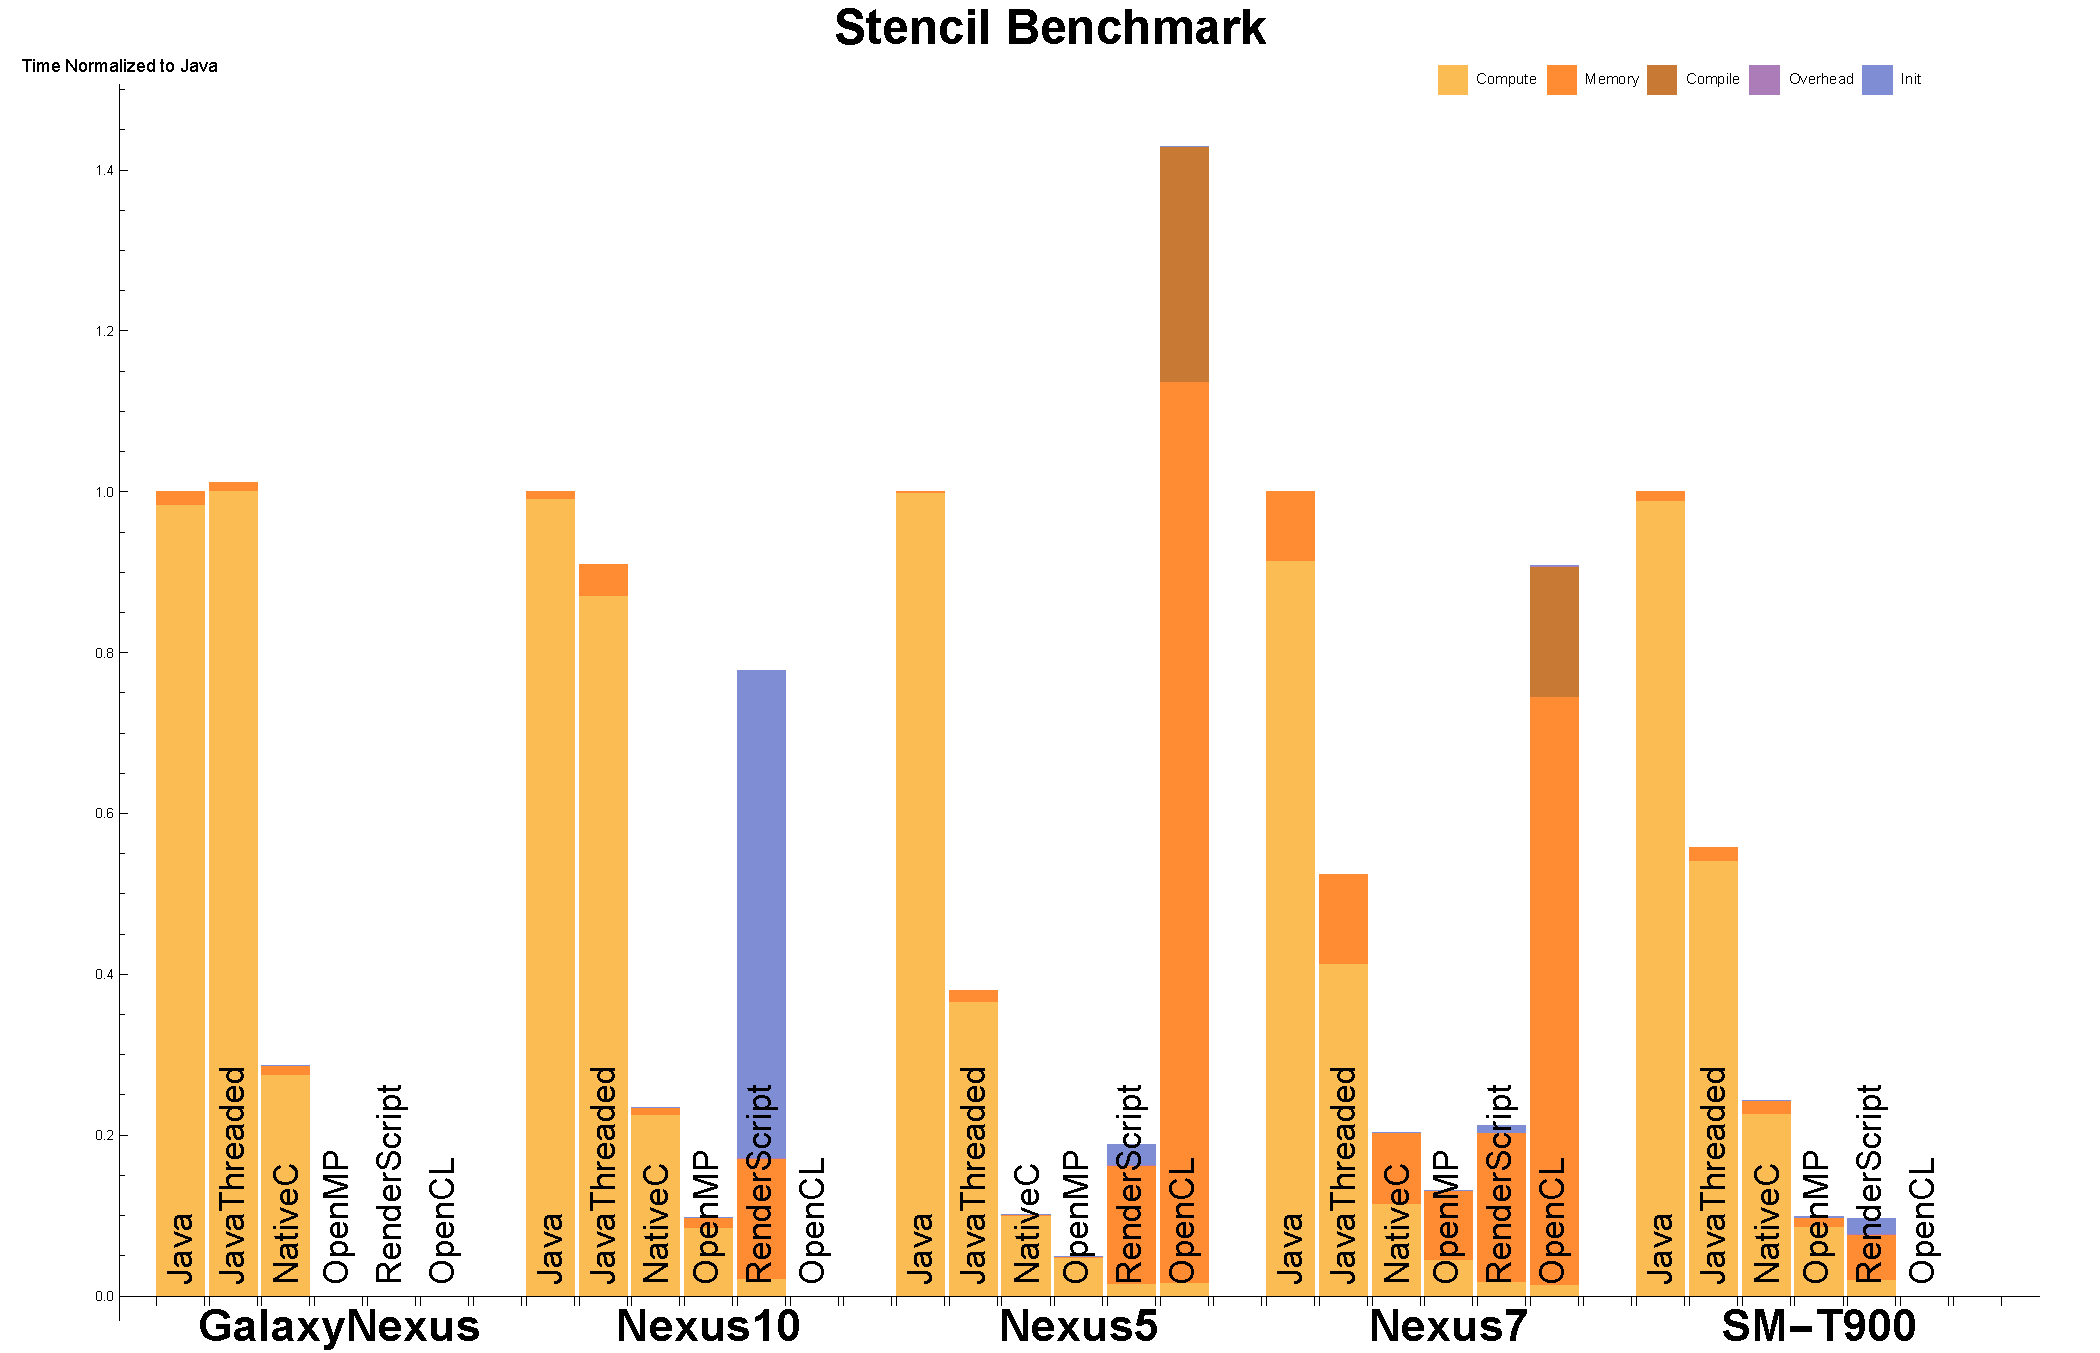
\includegraphics[width=0.9\textwidth]{data/Stencil_onecompute_time.pdf}
      \caption{Stencil}
      \label{fig:Stencil}
  \end{subfigure}

  \caption{Runtime across devices where kernel is executed once normalized to the Java execution time (lower is better). J : Java, JT : JavaThreaded, C : C with JNI, OMP: OpenMP, OCL : OpenCL, and RS : Renderscript.}
\end{figure*}
\FloatBarrier

The performance measurements are collected by measuring the time
  spent within each section of the code (as discussed in~\ref{design})
  while the device is plugged into the development machine.
Each compute part of an implementation is run $5$ times with the minimum
  presented.
We consider two cases --- one where the kernel code is run once and therefore
  the overhead (memory, compilation, and initialization) have an impact,
  and one where the kernel is run $100$ times (or $5$ for both TPACF and MRIQ)
  and the overhead has little impact.


For each device, the plot show the time to execute sections of the code normalized
  to the Java execution time.
These times correspond to the $x$-axis of the processor utilization times discussed
  in the previous section (e.g. figure~\ref{fig:loadVecAddSgemm}) --- Trepn is not
  running while collecting these timing results.

\subsubsection{VectorAdd}

\subsubsection{SGEMM}

\subsubsection{MRIQ}

\subsubsection{TPACF}

\subsubsection{Stencil}

\subsubsection{Histogram}

\begin{figure*}[t]

  \begin{subfigure}[b]{\textwidth}
          \centering
          
\includegraphics[width=0.4\textwidth]{data/legend.pdf}
  \end{subfigure}

  \begin{subfigure}[b]{0.5\textwidth}
      \centering
      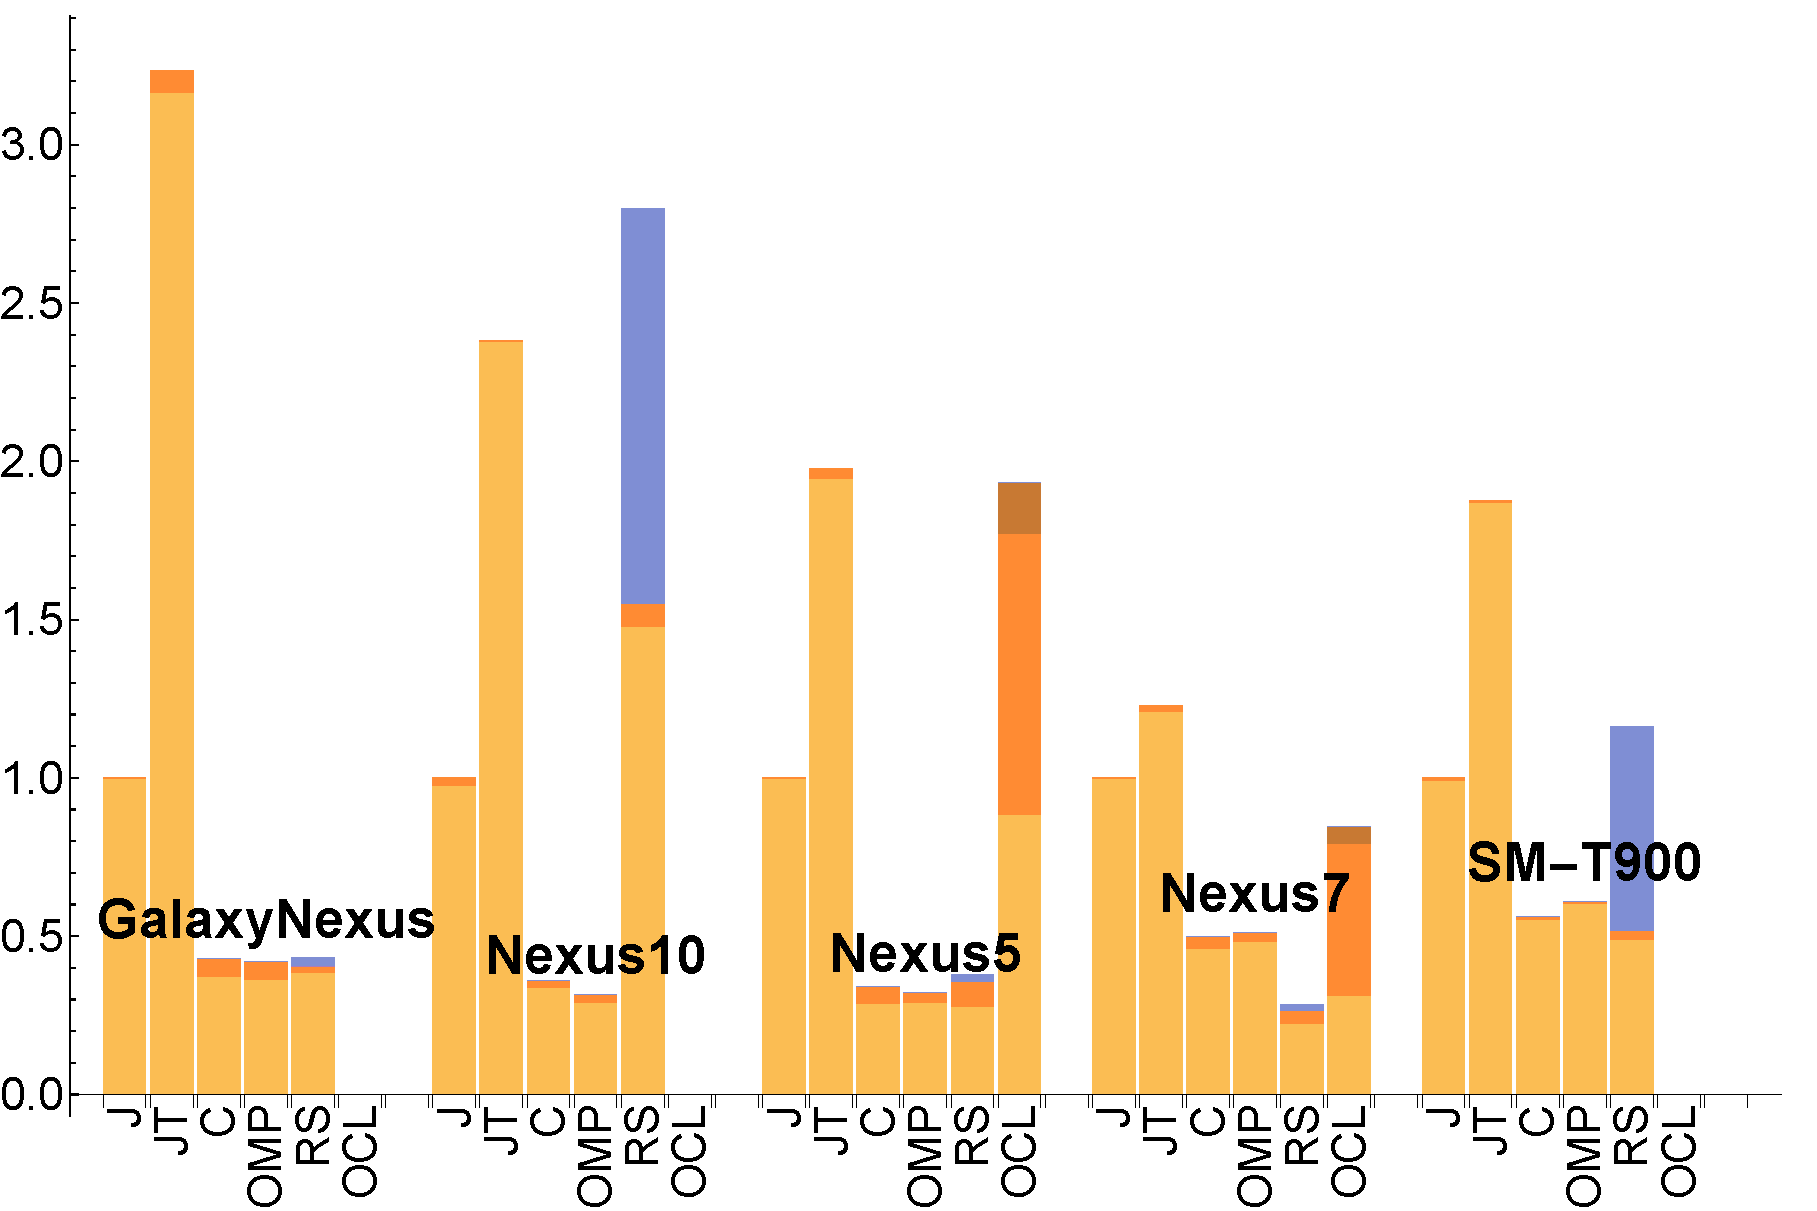
\includegraphics[width=0.9\textwidth]{data/VectorAdd_time.pdf}
      \caption{VectorAdd}\label{fig:vectoradd}
  \end{subfigure}
  \begin{subfigure}[b]{0.5\textwidth}
      \centering
      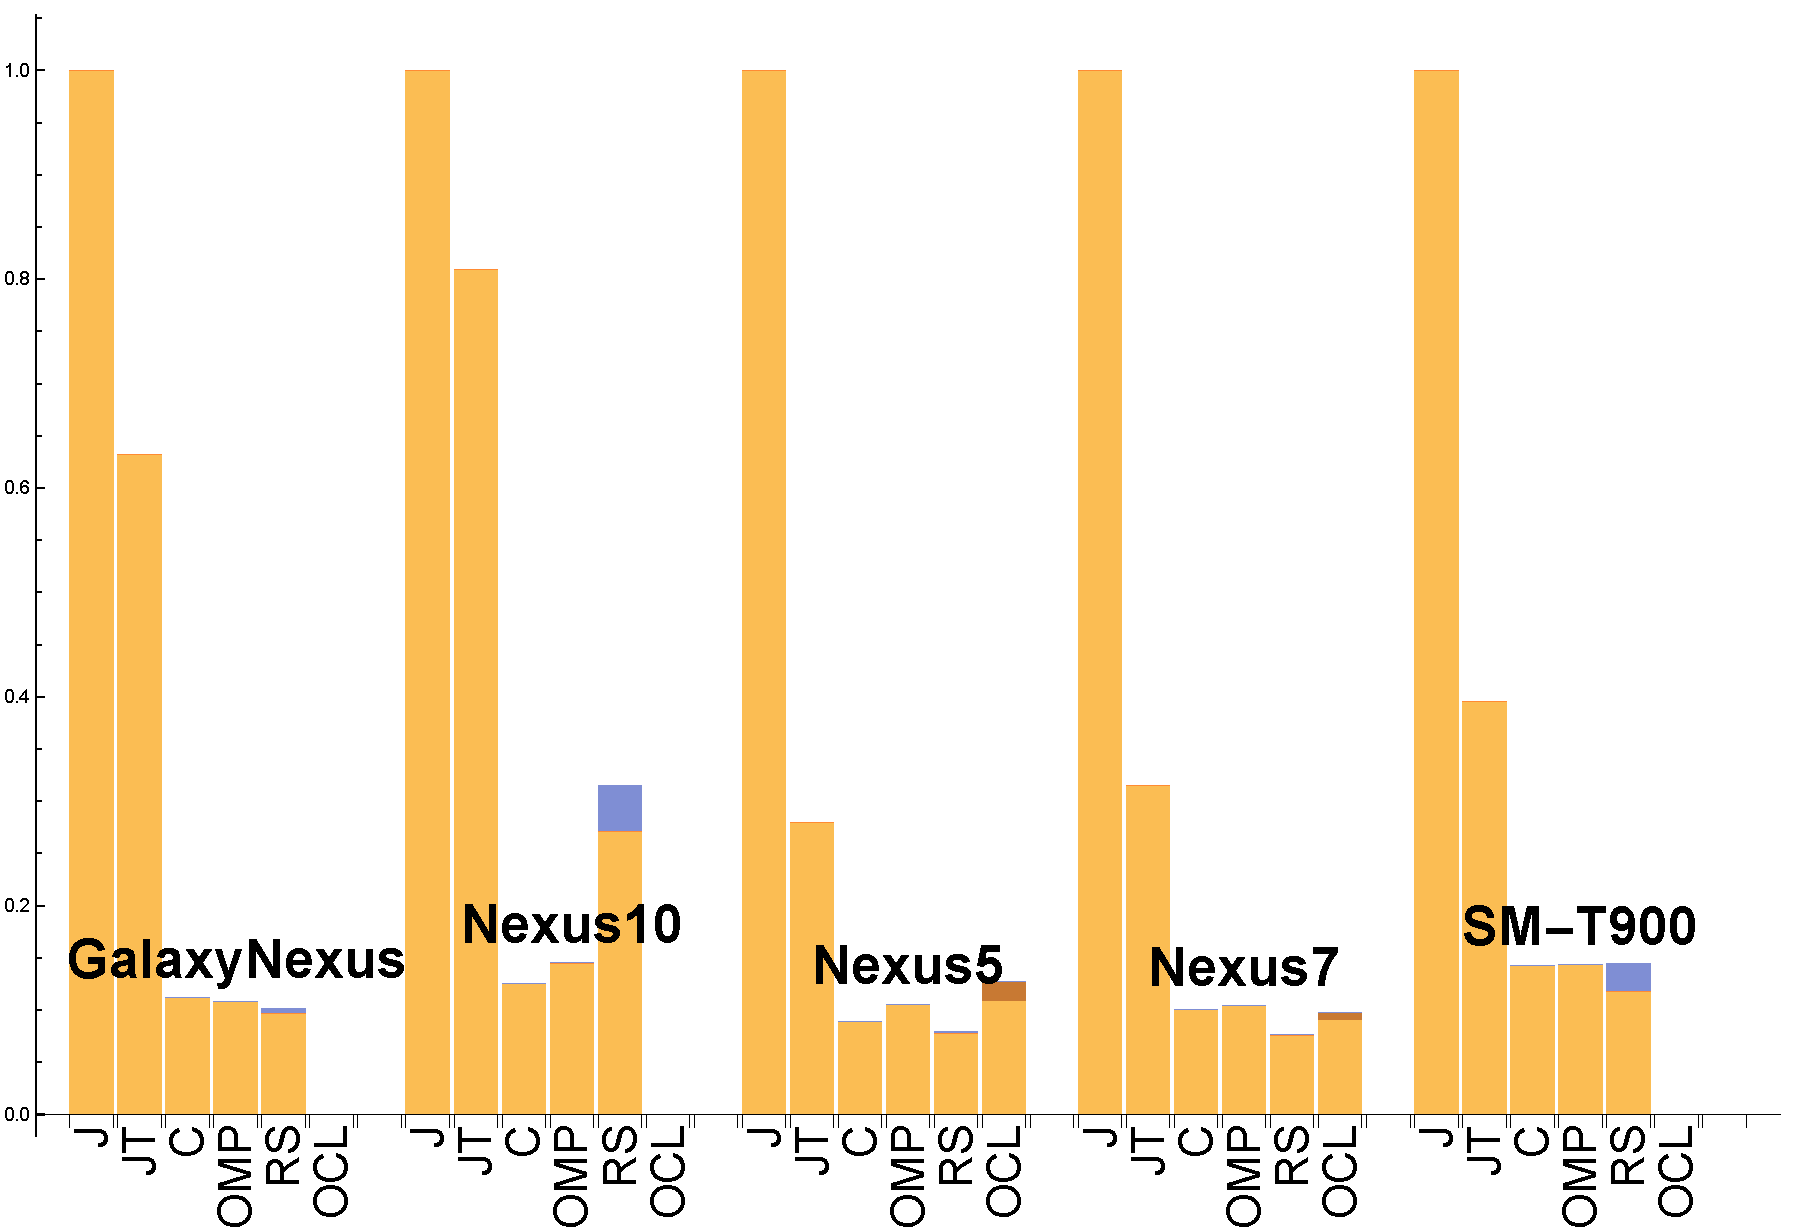
\includegraphics[width=0.9\textwidth]{data/Sgemm_time.pdf}
      \caption{Sgemm}\label{fig:Sgemm}
  \end{subfigure}

  \begin{subfigure}[b]{0.5\textwidth}
      \centering
      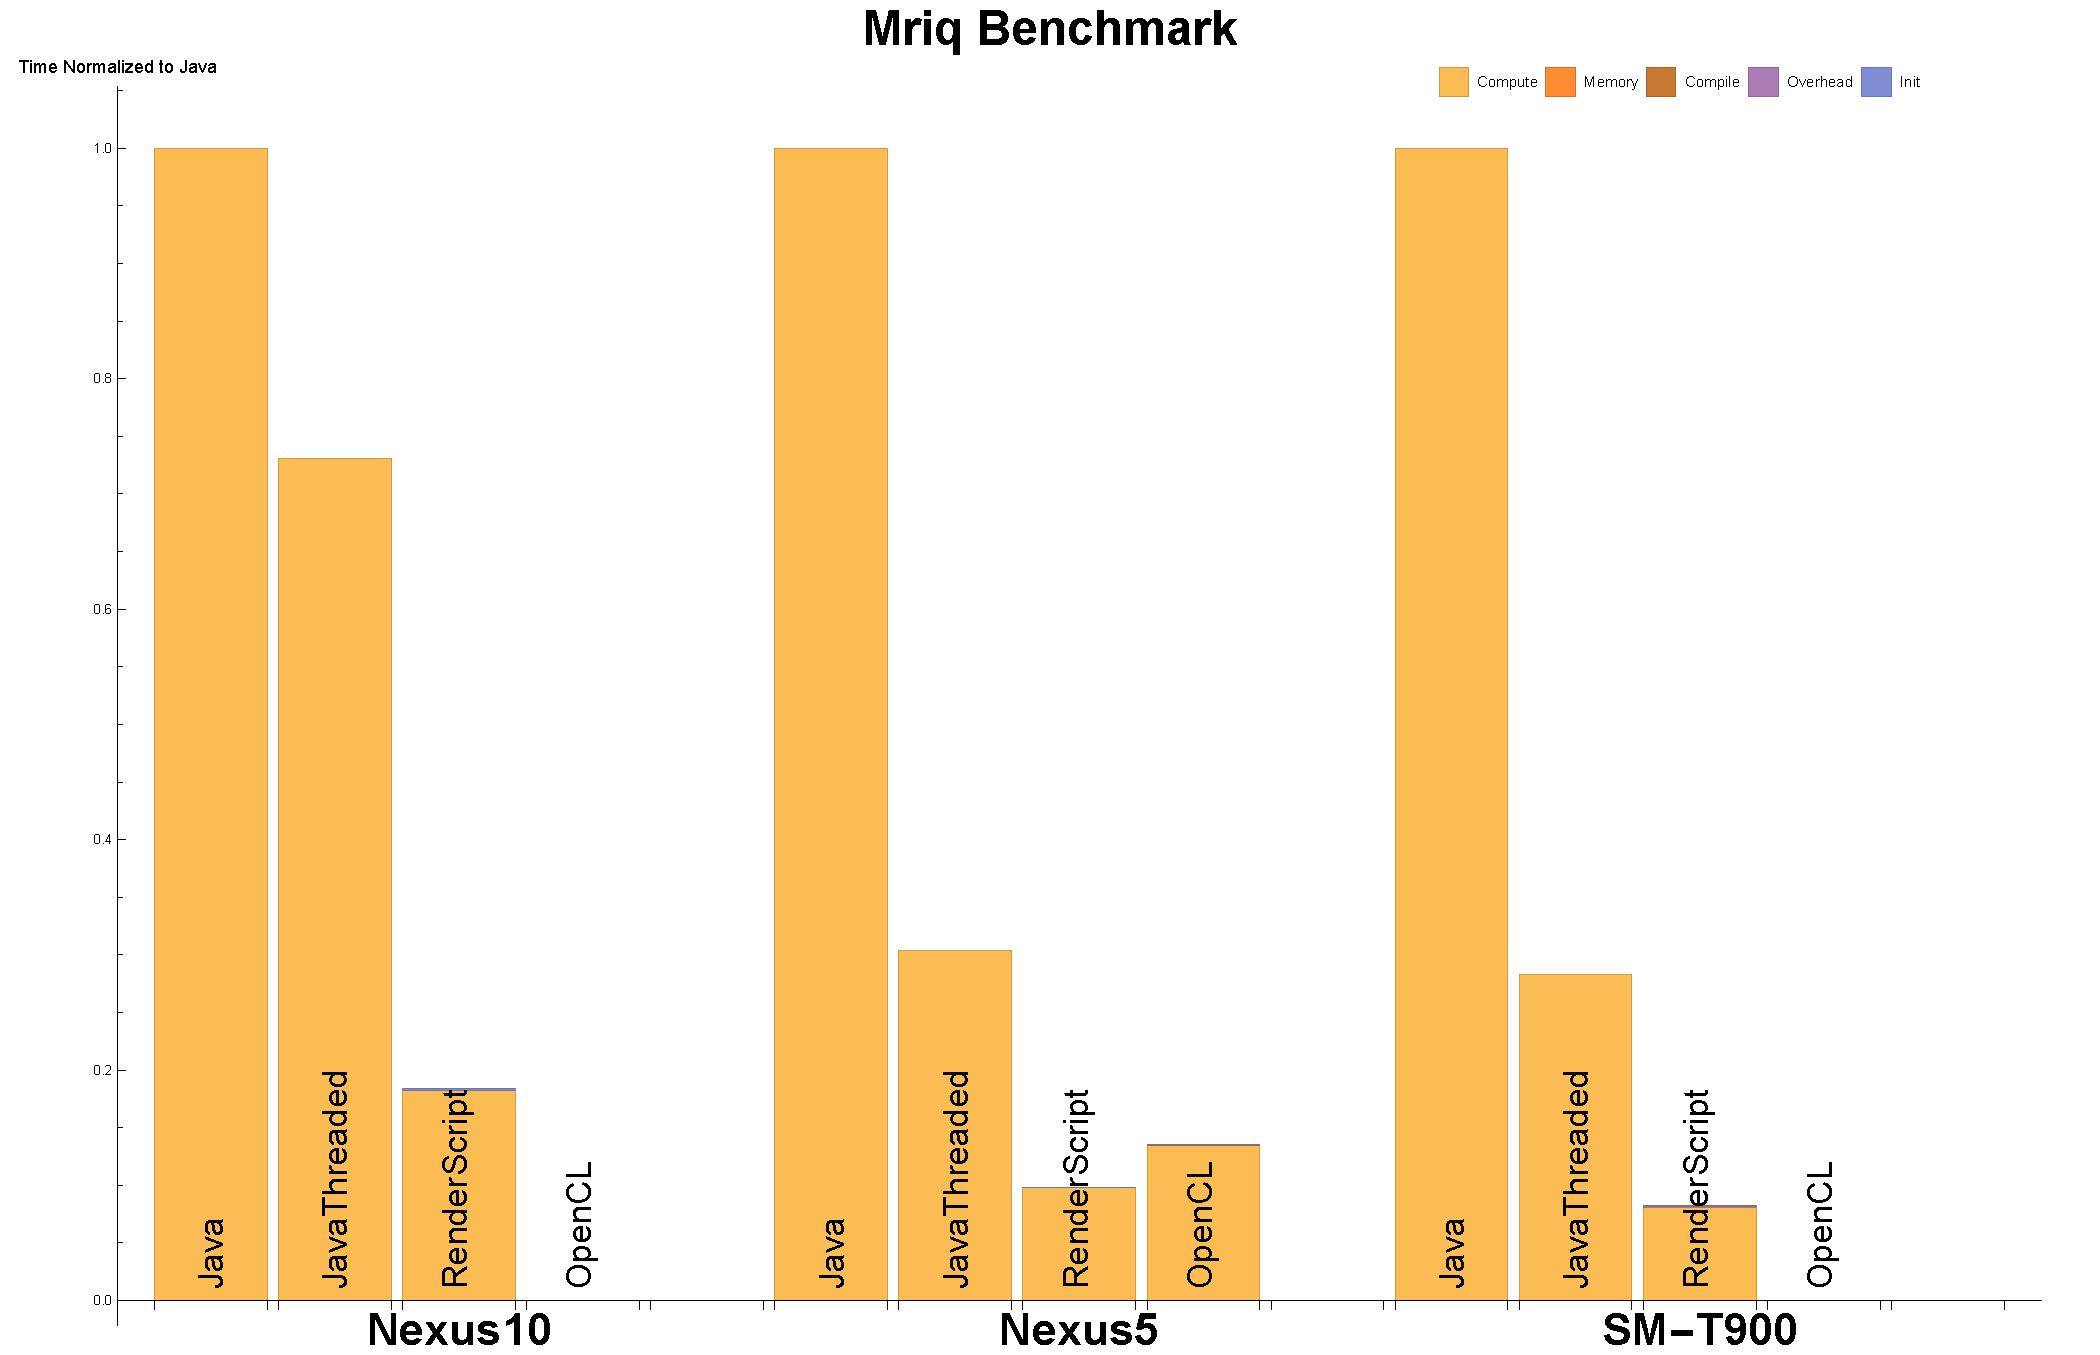
\includegraphics[width=0.9\textwidth]{data/Mriq_time.pdf}
      \caption{MRIQ}
      \label{fig:MRIQ}
  \end{subfigure}
  \begin{subfigure}[b]{0.5\textwidth}
      \centering
      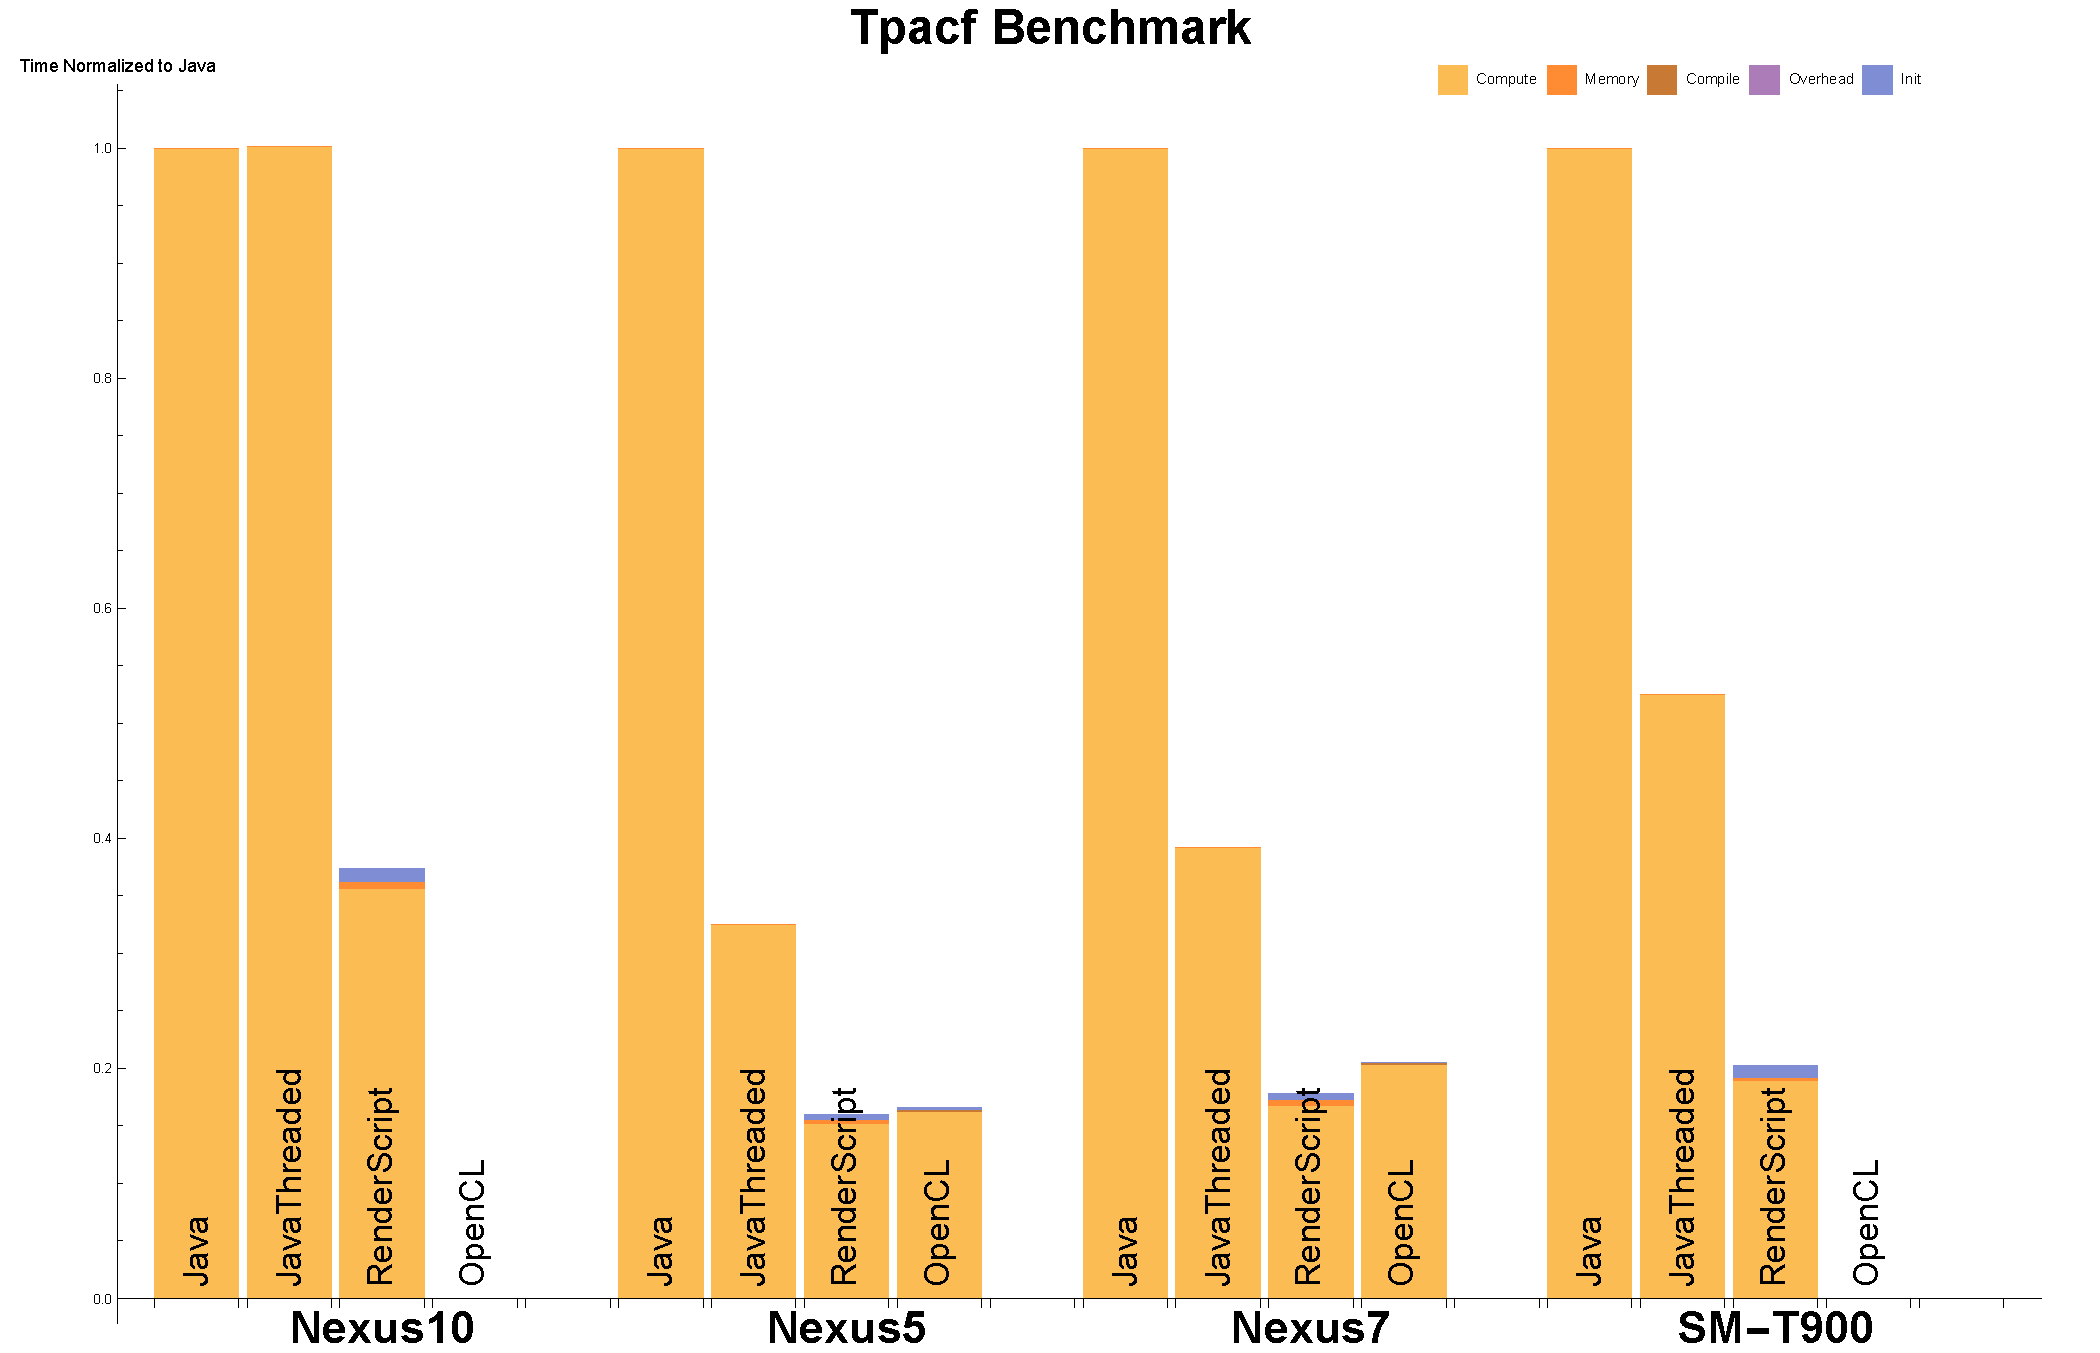
\includegraphics[width=0.9\textwidth]{data/Tpacf_time.pdf}
      \caption{TPACF}
      \label{fig:TPACF}
  \end{subfigure}

  \begin{subfigure}[b]{0.5\textwidth}
      \centering
      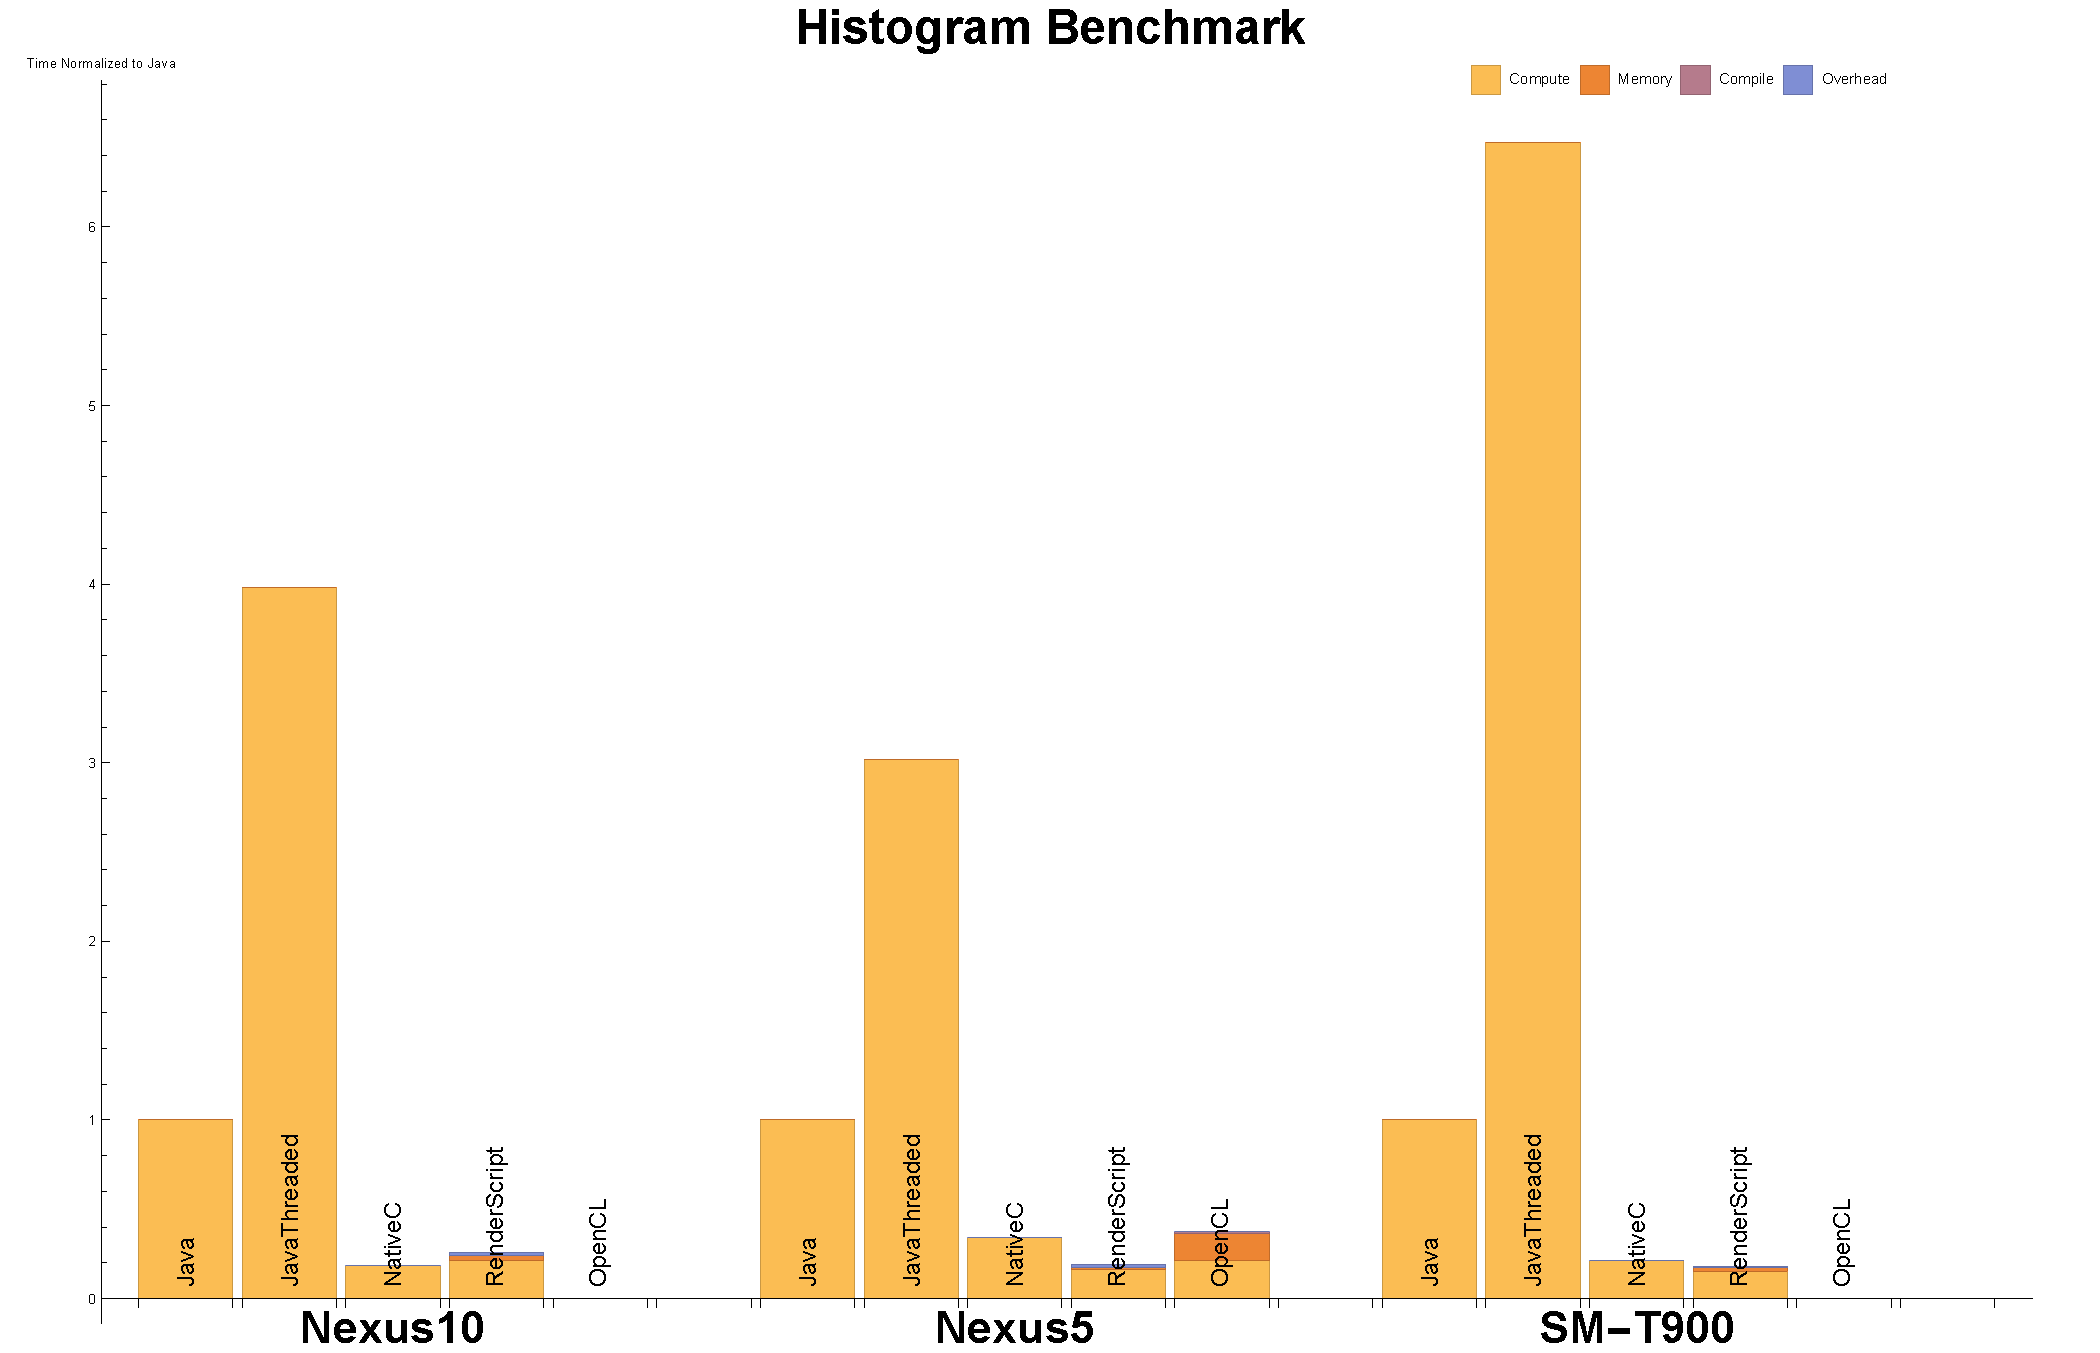
\includegraphics[width=0.9\textwidth]{data/Histogram_time.pdf}
      \caption{Histogram}\label{fig:histo}
  \end{subfigure}
  \begin{subfigure}[b]{0.5\textwidth}
      \centering
      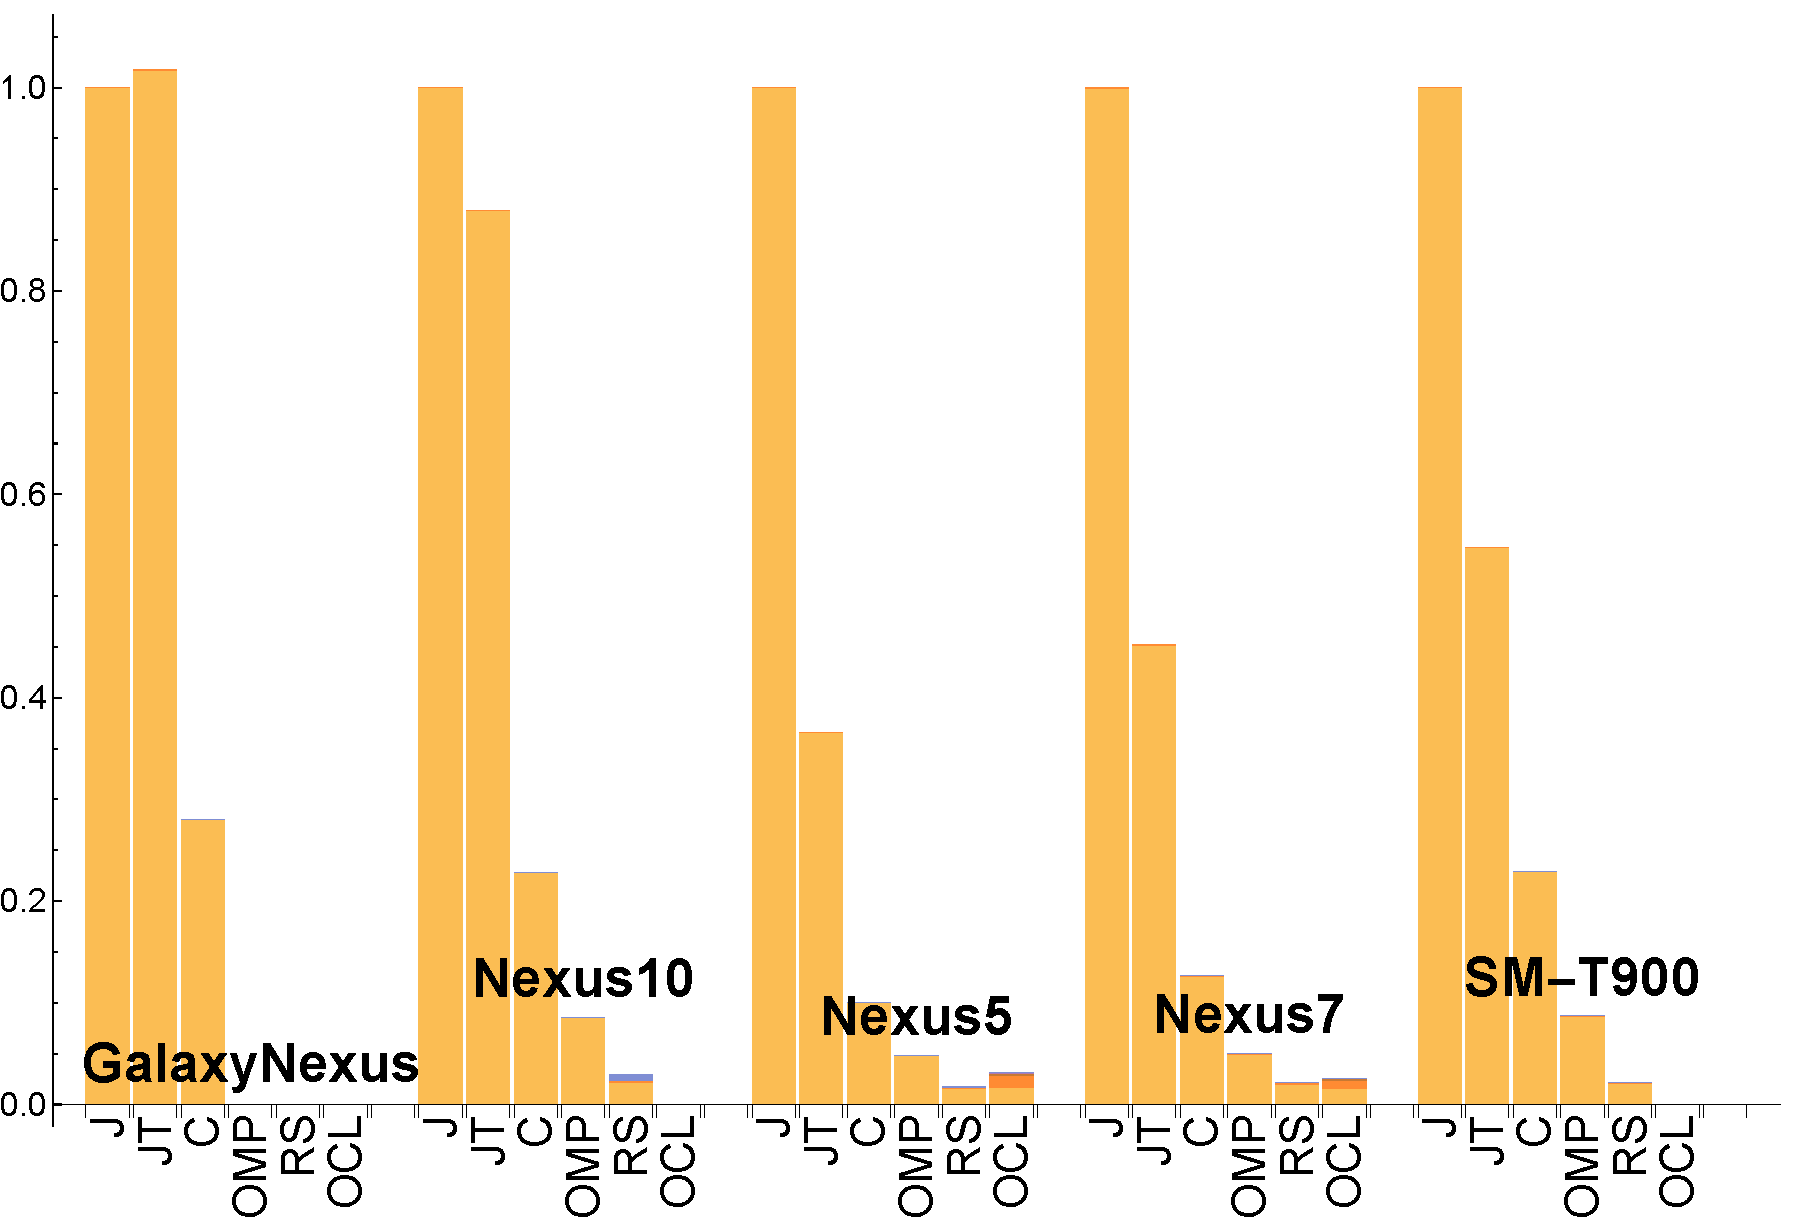
\includegraphics[width=0.9\textwidth]{data/Stencil_time.pdf}
      \caption{Stencil}
      \label{fig:Stencil}
  \end{subfigure}

  \caption{Runtime across devices where kernel is executed multiple times normalized to the Java execution time (lower is better). J : Java, JT : JavaThreaded, C : C with JNI, OMP: OpenMP, OCL : OpenCL, and RS : Renderscript.}
\end{figure*}
\FloatBarrier
